\documentclass{article}
\usepackage[utf8]{inputenc}
\usepackage{imakeidx}
\usepackage[italian]{babel}
\usepackage{graphicx}
\makeindex
\usepackage{float}
%\graphicspath{}
\title{Sintetizzatore di Frequenza}
\author{William Perri 4427140 }
\setlength{\parskip}{1em}
\renewcommand{\baselinestretch}{1.8}
%\DeclareGraphicsExtensions{.jpeg,.png}
\date{20/06/2020}

\begin{document}

\maketitle
Insegnamento di LABORATORIO DI ELETTRONICA A.A. 2019/20

\newpage
\tableofcontents
\newpage
\section{Introduzione}
\paragraph{Lo scopo del progetto consiste nel realizzare un sintetizzatore di frequenza basato su PLL (Phase Locked Loop).
Un PLL è composto da un rivelatore di fase, un filtro passa-basso ed un VCO (Voltage Controlled Oscillator).}
\paragraph{ Il progetto verrà dapprima simulato mediante software di simulazione ed in seguito realizzato in parte su breadboard ed in parte su una FPGA (Field Programmable Gate Array) Cyclone II, programmata mediante il software Quartus II sulla base del progetto realizzato su Digital Electronic Deeds.}


\newpage
\section{Descrizione del Progetto}

\paragraph{Come già detto nel capitolo precedente, il nostro sintetizzatore si baserà su un PLL il cui schema a blocchi è il seguente:\\ }

~\begin{figure}[!h]%Schema a blocchi PLL
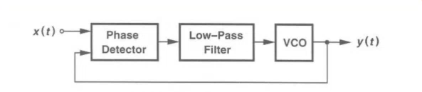
\includegraphics[scale=1.4]{PLLSchema.png} 
\caption{Schema a Blocchi PLL}
\label{fig:foo}
\end{figure}
~\begin{figure}[H]%Phase Detector
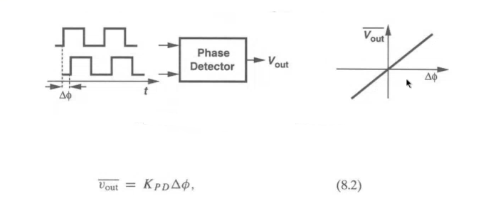
\includegraphics[scale=1]{PhaseDetect.png} 
\caption{Il Phase Detector lega la differenza di fase degli ingressi alla tensione d'uscita.}
\label{fig:foo}
\end{figure}




~\begin{figure}[!h]%Risposta al gradino
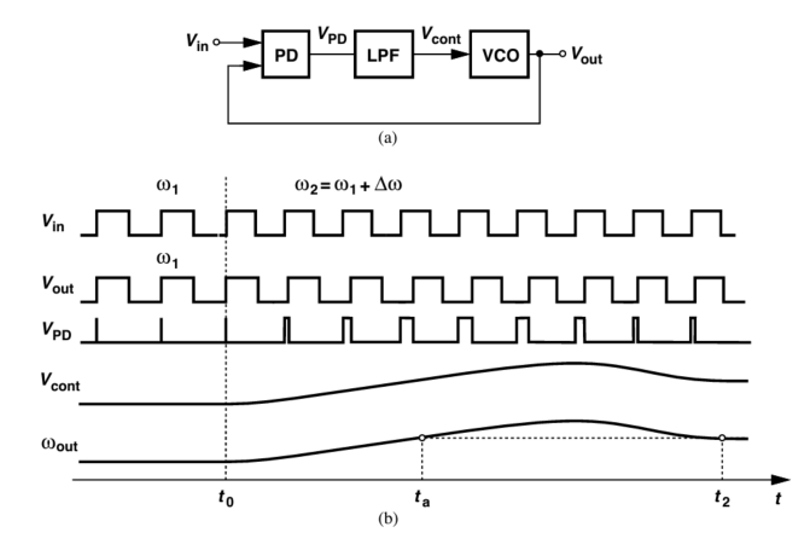
\includegraphics[scale=0.6]{PLLGradino.png} 
\caption{Risposta ad un gradino in frequenza}
\label{fig:foo}
\end{figure}
\paragraph{Analizzando la Figura 3, possiamo capire che se la tensione in uscita dal VCO è nulla (o al valore di riferimento), esso oscillerà ad una frequenza $\omega _{0}$, per modificare questa frequenza c'è necessità di cambiare la tensione di controllo $V_{CONT}$ in uscita dal LPF, la differenza di fase tra $V_{IN}$ e $V_{OUT}$ permette a $V_{PD}$ di generare un $\Delta V$ per modificare la frequenza del VCO. Il LPF deve "pulire" la tensione di controllo dai piccoli picchi che la tensione $V_{PD}$ avrebbe. 
Nell'istante $t_{0}$ la frequenza del segnale d'ingresso cambia, il periodo della Vin diminuisce, l'impulso VPD si allarga portando ad aumentare $V_{CONT}$, all'istante $t_{a}$, a causa delle dinamiche dell'anello, la tensione $V_{CONT}$ continua a salire, facendo aumentare conseguentemente la frequenza di oscillazione del VCO, fino a quando non si stabilizzerà a $\omega _{1}$ all'istante $t_{2}$.\\Andando ad esplicitare il LPF come un filtro del primo ordine, otteniamo quanto segue in Figura 4}
~\begin{figure}[!h]%Risposta al gradino
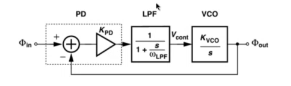
\includegraphics[scale=1.5]{Esplicitato.png} 
\caption{}
\label{fig:foo}
\end{figure}
\paragraph{Abbiamo la proporzionalità data dal PD, un polo dato dal LPF ed infine l'integratore che rappresenta il VCO. Possiamo calcolare le funzioni di trasferimento, sia ad anello aperto, sia ad anello chiuso ottenendo:\\$H_{0}(s)=K_{PD}\frac{1}{1+\frac{s}{\omega _{LPF}}}\frac{K_{VCO}}{s}$   e   $H(s)=\frac{K_{PD}K_{VCO}}{\frac{s^{2}}{\omega_{LPF}}}+s+K_{PD}K_{VCO}$}
\paragraph{Quanto detto fin'ora però presenta un problema: abbiamo\\ $\omega_{LPF}<<\omega_{IN}-\omega_{OUT}$, pertanto la differenza non riesce a passare nel LPF e il circuito non riesce ad agganciarsi. Per il nostro progetto quindi avremmo bisogno di un rivelatore che non tenga conto solo della fase ma anche delal frequenza: PFD (Phase-Frequency Detector, Figura 5).}
~\begin{figure}[!h]%Risposta al gradino
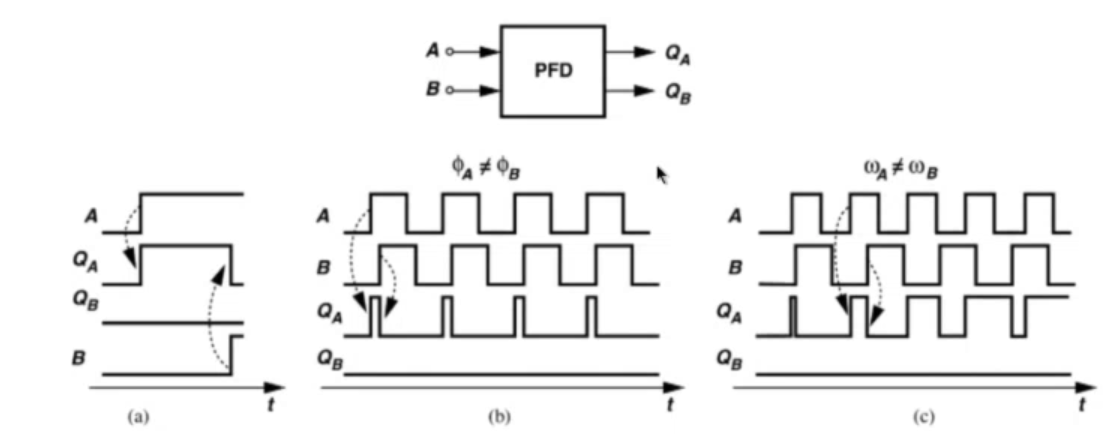
\includegraphics[scale=0.4]{PFD2.png} 
\caption{Schema di un PFD}
\label{fig:foo}
\end{figure}
\paragraph{Se il fronte di salita del segnale $A$ arriva prima del fronte del segnale $B$, il segnale d'uscita $Q_A$ va a 1 fino a quando non arriva il fronte di B, quindi la larghezza dell'impulso di $Q_A$ è proporzionale alla differenza di fase tra i due segnali. Al contrario ovviamente se $B$ fosse in anticipo rispetto ad $A$, accadrebbe la medesima cosa però sul segnale $Q_B$.
Questo dispositivo è stato implementato come si può vedere in Figura 6.
}
~\begin{figure}[!h]%Risposta al gradino
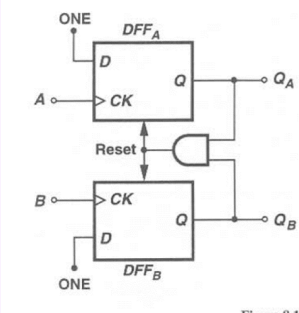
\includegraphics[scale=0.8]{PFD.png} 
\caption{Realizzazione di un PFD}
\label{fig:foo}
\end{figure}
\paragraph{A questo punto andiamo a realizzare un pompa di carico da aggiungere in cascata al PFD}
~\begin{figure}[!h]%Risposta al gradino
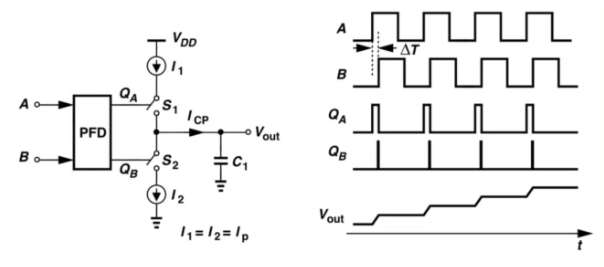
\includegraphics[scale=0.8]{CP.png} 
\caption{Rappresentazione simbolica della Charge Pump}
\label{fig:foo}
\end{figure}
\paragraph{Se $Q_A$ è a 1, chiude lo switch $S_1$, facendo caricare il condensatore $C_1$, facendo aumentare la frequenza del VCO.
L'uscita $Q_B$ invece fa scaricare lievemente il condensatore, in quanto gli impulsi di $Q_B$ sono molto più stretti di quelli di $Q_A$, il condensatore $C_1$ sostituisce anche il LPF, generando però un problema, la nuova funzione di trasferimento è quella in Figura 8}
~\begin{figure}[!h]%Risposta al gradino
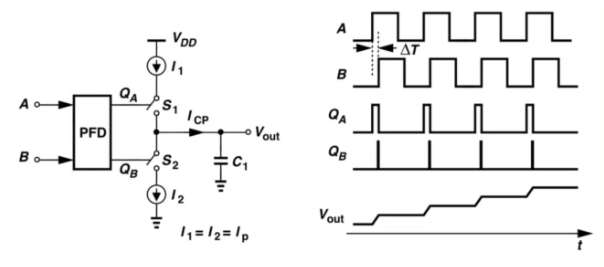
\includegraphics[scale=0.8]{CP.png} 
\caption{Funzione di Trasferimento}
\label{fig:foo}
\end{figure}
\paragraph{Questa presenta due poli immaginari nell'origine, rendendo così il sistema instabile. A questo punto per ovviare a questo problema si deve per forza di cose aggiungere uno zero in zero alla funzione di trasferimento, aggiungendo un resistore prima del condensatore.
Il fattore di smorzamento diventa >0 , il margine di fase che in precedenza era nullo, ora anch'esso è aumentato.  
Questo non è l'unico aspetto positivo di questa realizzazione, perché anche all'aumentare del guadagno, abbiamo che il margine di fase aumenta ulteriormente di conseguenza (Figura 9), migliorando la stabilità.}
~\begin{figure}[!h]%Risposta al gradino
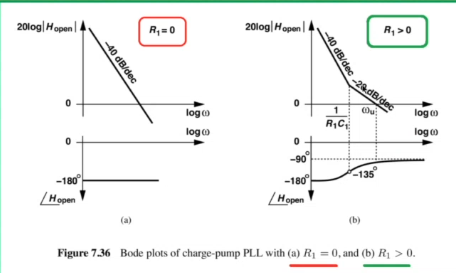
\includegraphics[scale=0.8]{ZPFD.png} 
\caption{Il margine di fase aumenta}
\label{fig:foo}
\end{figure}
\paragraph{A questo punto possiamo inserire un divisore di frequenza.}
~\begin{figure}[!h]%Risposta al gradino
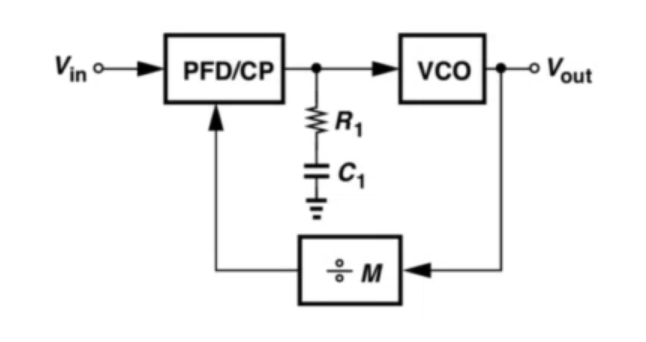
\includegraphics[scale=0.6]{DivM.png} 
\caption{PLL con pompa di carico e divisore per M}
\label{fig:foo}
\end{figure}
\paragraph{Per completare il nostro progetto bisognerà dimensionare $I_P,R_1,C_1$, il $K_VCO$ sarà noto in quanto parametro di costruzione.
Con l'inserimento del divisore per e portando la nuova $H(S)$ nella forma "canonica" abbiamo $\zeta=\frac{R_1}{2}\sqrt{\frac{I_P K_{VCO}C_1}{2\pi M}}$ e }

$\omega _n= \sqrt  {   \frac{I_pK_{VCO}C_1}{2\pi M}   }$ 

\paragraph{Per il nostro progetto dovremo tenere conto delle richieste che sono:$f_{OUT}=1 MHz$\\$f_{REF}=10 kHz$\\$M=100 (80\div150)$.\\Il VCO che utilizzeremo sarò il 74LS624.}
~\begin{figure}[!h]%Risposta al gradino
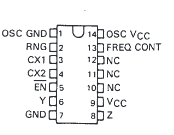
\includegraphics[scale=1]{74LS.png} 
\centering
\caption{Pinout del VCO}
\label{fig:foo}
\end{figure}
~\begin{figure}[!h]%Risposta al gradino
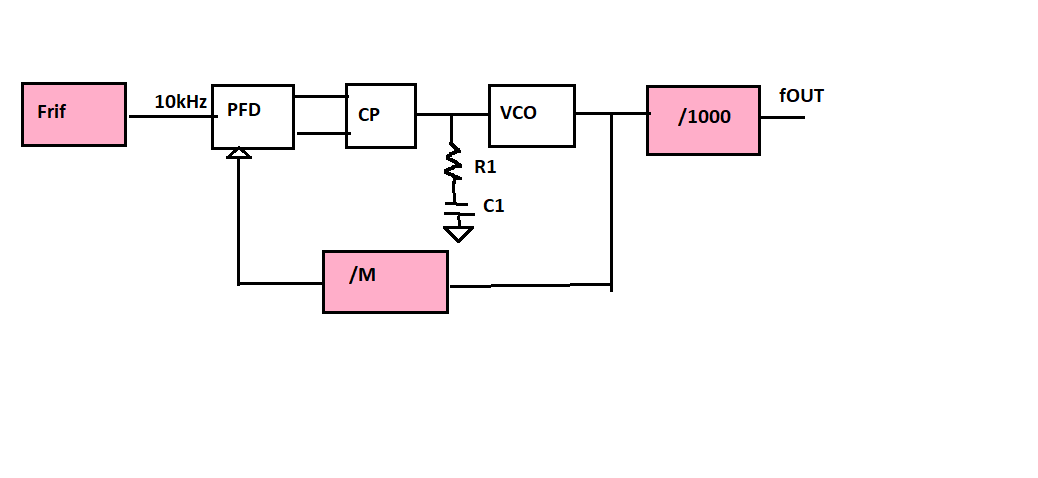
\includegraphics[scale=0.4]{SCH.png} 
\centering
\caption{Schema a blocchi dei dispositivi da realizzare.}
\label{fig:foo}
\end{figure}
\paragraph{Il divisore per M, realizzato sull'FPGA, presenterà uno dip switch, da 8 interruttori, per selezionare il numero M. Il DIP switch verrà collegato a due array di resistenze, quando uno singolo switch sarà ON, l'ingresso sulla FPGA verrà visto come basso, perché collegato a massa(attraverso le due resistenze), mentre se lo switch è su OFF, l'ingresso della FPGA vede il valore logico alto (3.3V)}
\newpage
\section{Realizzazione}
\paragraph{Viene descritto come si è realizzato il sistema finale (tramite simulatore o come realizzazione pratica)}

\newpage
\section{Risultati}
\paragraph{Sono  raccolti  di  risultati  più  significativi,  intesi  come  prestazioni  del  circuito  finale,  in  modo  sufficiente per poterlo caratterizzare adeguatamente}

\newpage
\section{Conclusioni}
\paragraph{Si riassumono i punti salienti del progetto svolto}

\newpage
\section{Riferimenti}
\paragraph{Contiene  sia  la  bibliografia  (libri,  articoli,  manuali)  sia  i  siti  web  eventualmente  impiegati  durante il progetto}
\end{document}
